\chapter[Grundlagen]{Grundlagen}

Ziel dieses Kapitels ist die Erläuterung von notwendigen Konzepten zur weiteren Betrachtung des Themas Integration der Data Science in Organisationen und Abteilungen.
Dazu wird in diesem Kapitel besonders auf die grundlegende Thematik der Data Science eingegangen.

Wie in der Problemstellung identifiziert, steigt das Interesse an der Aufzeichnung und Verarbeitung von Daten innerhalb von Organisationen. 
Da hierfür folglich qualifiziertes Fachpersonal benötigt wird, nimmt auch die Rolle des Data Scientist an Wert für Unternehmen zu. \footcite[Vgl.][S. 1]{Fabijan.2017}
Aufgabe dieser Rolle ist es, an Datenanwendungen zu arbeiten, welche eine zeitnahe signifikante Auswirkung auf das Geschäftsmodell verursachen. \footcite[Vgl.][S. 12]{Patil.2011}
Data Science im Allgemeinen wird häufig mit einem Prozess in Verbindung gebracht, welcher durch Einsatz von Techniken des maschinellen Lernens wichtige Erkenntnisse aus Daten ableitet. \footcite[Vgl.][S. 1]{Zhang.2020b}
van der Aalst definierte im Jahr 2016 das Feld der Data Science wie folgt: \footcite[Vgl.][S. 10]{vanderAalst.2016}

% \begin{quotation}
%     \textit{
%     Data science is an interdisciplinary field aiming to turn data into real value.
%     Data may be structured or unstructured, big or small, static or streaming.
%     Value may be provided in the form of predictions, automated decisions, models learned from data, or any type of data visualization delivering insights.
%     Data science includes data extraction, data preparation, data exploration, data transformation, storage and retrieval, computing infrastructures, various types of mining and learning, presentation of explanations and predictions, and the exploitation of results taking into account ethical, social, legal, and business aspects.    
%     }
% \end{quotation}

\begin{quotation}
    Data Science ist ein interdisziplinäres Feld mit dem Ziel Wert aus Daten zu generieren.
    Daten können dabei in strukturierter oder unstrukturierter Form, in großer oder geringer Menge, statisch oder nur in Echtzeit vorliegen.
    Wert entsteht durch Vorhersagen, automatisierten Entscheidungen, optimierten Modellen oder Visualisierungen, welche Erkenntnisse erzeugen.
    Data Science inkludiert die Extraktion, Vorverarbeitung, Erkundung, Transformation, Speicherung und den Erhalt von Daten sowie Recheninfrastruktur, Arten des Lernens, das Präsentieren von Erklärungen und die Nutzung von Erkenntnissen unter ethischen, sozialen, rechtlichen und geschäftlichen Aspekten.
\end{quotation}

Die Definition betrachtet die drei wichtigen Aspekte der Daten, des Wertbeitrags und der Aufgabenbereiche.
Folgend werden die einzelnen Aspekte, ausgeschlossen des bereits im vorherigen Kapitel behandelten Wertbeitrags, detaillierter ausgeführt.

% Daten
Aus der Definition lassen sich bereits einige Charakteristika von Daten hinsichtlich Form, Menge und Persistenz erkennen.
In der Literatur werden besonders im Bereich von \textit{Big Data} die 5 V's von Daten thematisiert.
Übersetzt beschreiben sie die Charakteristika Volumen, Geschwindigkeit, Wahrheit, Vielfalt und Wert. \footcite[Vgl.][S. 1]{Naeem.2022}
Ausprägungen dieser Merkmale lassen sich wie folgt zuordnen: Volumen - Number of Bytes, Geschwindigkeit - static or real time, Richtigkeit - Grad der Vorurteilsbelastung, Vielfalt - strukturiert oder unstrukturiert, Wert - Leistungspotenzial der Daten.
Von diesen Charakteristika liegt jedoch global betrachtet der Großteil der Daten in unstrukturierter Form, bspw. als Text, Bild oder Audio, vor. \footcite[Vgl.][S. 4]{vanderAalst.2016}

% Disziplin / Aufgabenbereich
Die Disziplin der Data Science entwickelte sich aus der Statistik und der Kombination vieler verwandter Disziplinen, welche selbst unter sich Überschneidungen aufweisen und in ihrem Einfluss auf die Data Science variieren. \footcite[Vgl.][S. 12]{vanderAalst.2016}
Die verwandten Wissenschaftsbereiche sind dabei in Abbildung 2.1 aufgezeigt. \footcite[Vgl.][S. 12]{vanderAalst.2016}

\begin{figure}[htb]
    \centering
    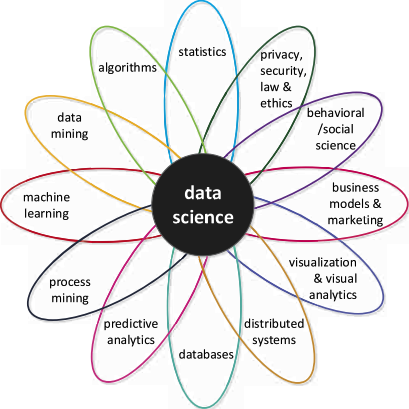
\includegraphics[width=0.5\textwidth]{graphics/ds_disciplines.png}
    \caption{Disziplinen der Data Science}
    \label{fig:data science disciplines}
\end{figure}

Anwendung der Data Science und deren Subdisziplinen findet sich in der Bearbeitung von datengetriebenen Problemstellungen der vier Kategorien: Berichterstattungen, Diagnosen, Vorhersagen und Empfehlungen. \footcite[Vgl.][S. 10]{vanderAalst.2016}
Als Arbeitsablauf dieser Bearbeitung wird in der Literatur häufig ein Prozessmodel mit drei Phasen und bis zu zehn Schritten beschrieben, welcher die Phasen der Datenvorbereitung, der Modellentwicklung und dessen Bereitstellung involviert. \footcite[Vgl.][S. 1]{Zhang.2020b}
Dabei ist es sinnvoll, je nach Anwendung und Problemstellung verschiedene Phasen zu fokussieren.
Beispielsweise sind zur Berichterstattung die Datenvorbereitung und Bereitstellung der Erkenntnisse zu fokussieren, da häufig kein explizites Modell zu entwickeln ist.
Hingegen werden bei der Erstellung von Vorhersagen und Empfehlungen akkurate Modelle benötigt, um die Richtigkeit der Vorhersagen und Empfehlungen zu garantieren.
Konkrete Aufgaben in der Data Science Rolle umfassen das Bereinigen und Vereinen von Datensätzen, die Visualisierung von Daten oder die Entwicklung umfangreicher Softwaretools zur Verarbeitung von Daten. \footcite[Vgl.][S. 13]{Patil.2011}
Das Produkt der Phasen und konkreten Aufgaben kann dabei als analytisches System in einer Organisation betrachtet werden, welches sich aus der Infrastruktur, den Modellen und insgesamt deren Betrieb zusammensetzt. \footcite[Vgl.][S. 22]{Grossman.2014}
Neben dem bekanntesten Anwendungsbereich der Kundenintelligenz kommen derartige analytische Systeme auch im Bereich von Lieferketten- und Qualitätsmanagement sowie Risikoanalyse und Betrugsdetektion zum Einsatz. \footcite[Vgl.][S. 221ff.]{Elgendy.2014}
% Tools
% Zur Umsetzung dieser Aufgaben der unterschiedlichen Phasen werden existieren eine Vielzahl von Werkzeugen und Technologien.
